\section{Introduction}

Techniques for analysing the dynamic dependency structure of programs have been fruitful, with applications ranging from information-flow security~\cite{sabelfeld03} and optimisation~\cite{kildall73} to debugging and program comprehension~\cite{weiser81,delucia96}. There are, however, few methods suitable for fine-grained analysis of richly structured outputs, such as data visualisations and multidimensional arrays. Dataflow analyses \cite{reps95} tend to focus on analysing variables rather than parts of structured values. Where-provenance~\cite{buneman01} and related data provenance techniques are fine-grained, but specific to relational query languages. Taint tracking \cite{newsome05} is also fine-grained, but works forwards from input to output. For many applications, it would be useful to be able to focus on a particular part of a structured output, and have an analysis isolate the input data pertinent only to that substructure.

This is a need that increasingly arises outside of traditional programming. Journalists and data scientists use programs to compute charts and other visual summaries from data, charts which must be interpreted by colleagues, policy makers and lay readers alike. Interpreting a chart correctly means understanding what the components of the visualisation actually \emph{represent}, i.e.~the mapping between data and visual elements. But this is a hard task, requiring time and expertise, even with access to the data and source code used to create the visualisation. In practice it is easy for innocent (but devastating) mistakes such as transposing two columns of data to go unnoticed~\cite{miller06}.

\todo{signpost the next two sections}

\subsection{Linking structured outputs to structured inputs}

The situation would be much improved if a computed artefact such as a chart or summary allowed a user to explore the relationship to the underlying data through the artefact itself, revealing the relevant data on a need-to-know basis. For example in \figref{introduction:data-linking} below, selecting a particular bar in the bar chart should present the user with a tabular summary of the data relevant to that bar:

\begin{figure}[H]
   \begin{subfigure}{0.35\textwidth}
      \small
      \begin{lstlisting}
let input = [ ... ]
let b1 = input |> filter (fun c -> c.country = "AB")
let b2 = input |> filter (fun c -> c.country = "CD")
in barchart [b1; b2]
      \end{lstlisting}
      \todo{TP: Modified code so that it filters input data. This shows we need to prpoagate information through our code (Altair would have to filter in the Altair DSL)}
   \end{subfigure}
   \begin{subfigure}{0.63\textwidth}
      {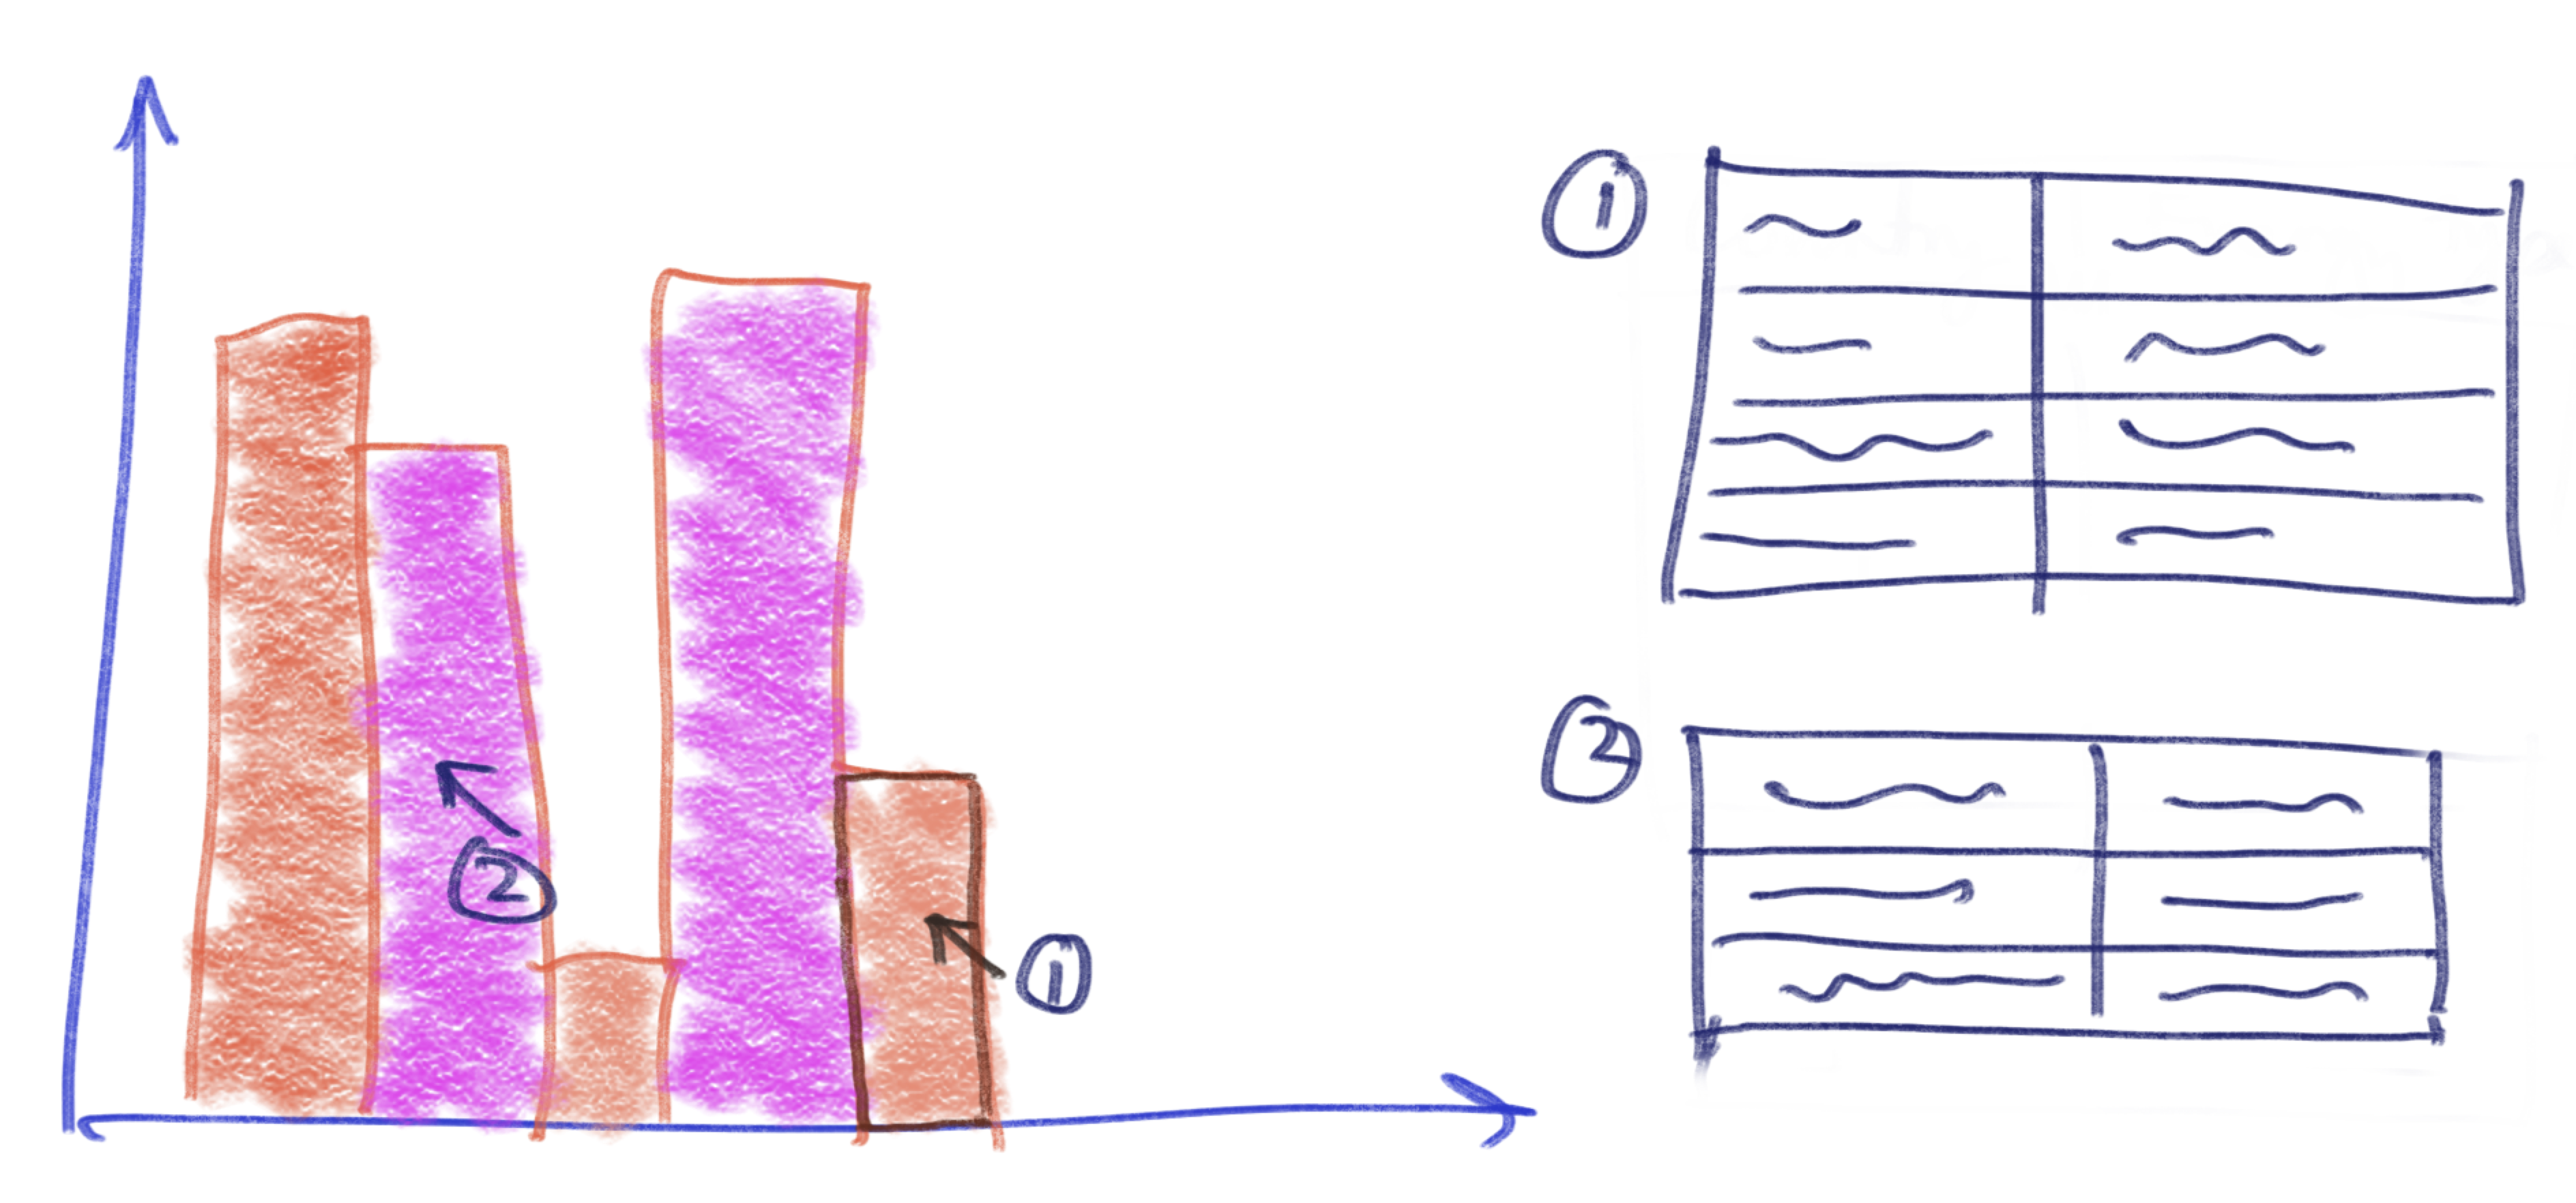
\includegraphics[scale=0.05]{fig/example/data-linking.png}}
   \end{subfigure}
   \caption{Linking structured outputs to structured inputs}
   \label{fig:introduction:data-linking}
\end{figure}

Indeed, visualisation designers do sometimes create ``data-linked'' artefacts like these by hand, such as Nadieh Bremer's award-winning visualisation of population density growth in Asian cities~\cite{bremer15}. But crafting such things by hand is a significant undertaking, requiring intimate knowledge of the computational relationship between chart and data, and programming effort to expose that information to the reader. Manual approaches are also error-prone and need to be changed whenever the application logic changes. A library-based approach would improve on this, but would only provide data linking for solutions expressible using the combinators provided by the library.

An alternative is to frame this as a program analysis problem. We want to be able to focus on a particular visual element, such as a bar in the bar chart above, and determine the inputs that contribute to it. This is a matter of selecting a part of the structured output and performing some kind of backwards analysis that identifies the relevant data. The advantage of this approach is that data linking comes ``for free'', and the data scientist or visualisation designer is able to code their analyses as pure functions of the data using the full expressive power of the language.

\subsection{Linking structured outputs to other structured outputs}

\todo{Make this an evolution of previous example.} It is also common to use more than one view to present distinct but related aspects of data. In this situation the user should be able to focus on (select) a visual element in one chart or other structured output and have those elements of a different chart which were computed using related inputs be automatically selected. For example in \figref{introduction:vis-linking} below, selecting a bar on the left automatically should select all the related visual elements on the right. This is a well-recognised use case in data visualisation, where it is called \emph{brushing and linking}~\cite{becker87}. Geospatial applications like GeoDa~\cite{anselin06} and charting libraries like Plotly support brushing and linking, but they tend to be baked into specific applications, or require programmer effort and therefore must be anticipated in advance by the chart designer. Moreover these applications and libraries provide no direct way for the reader to see the common data which explains why elements are related.

\begin{figure}[H]
   {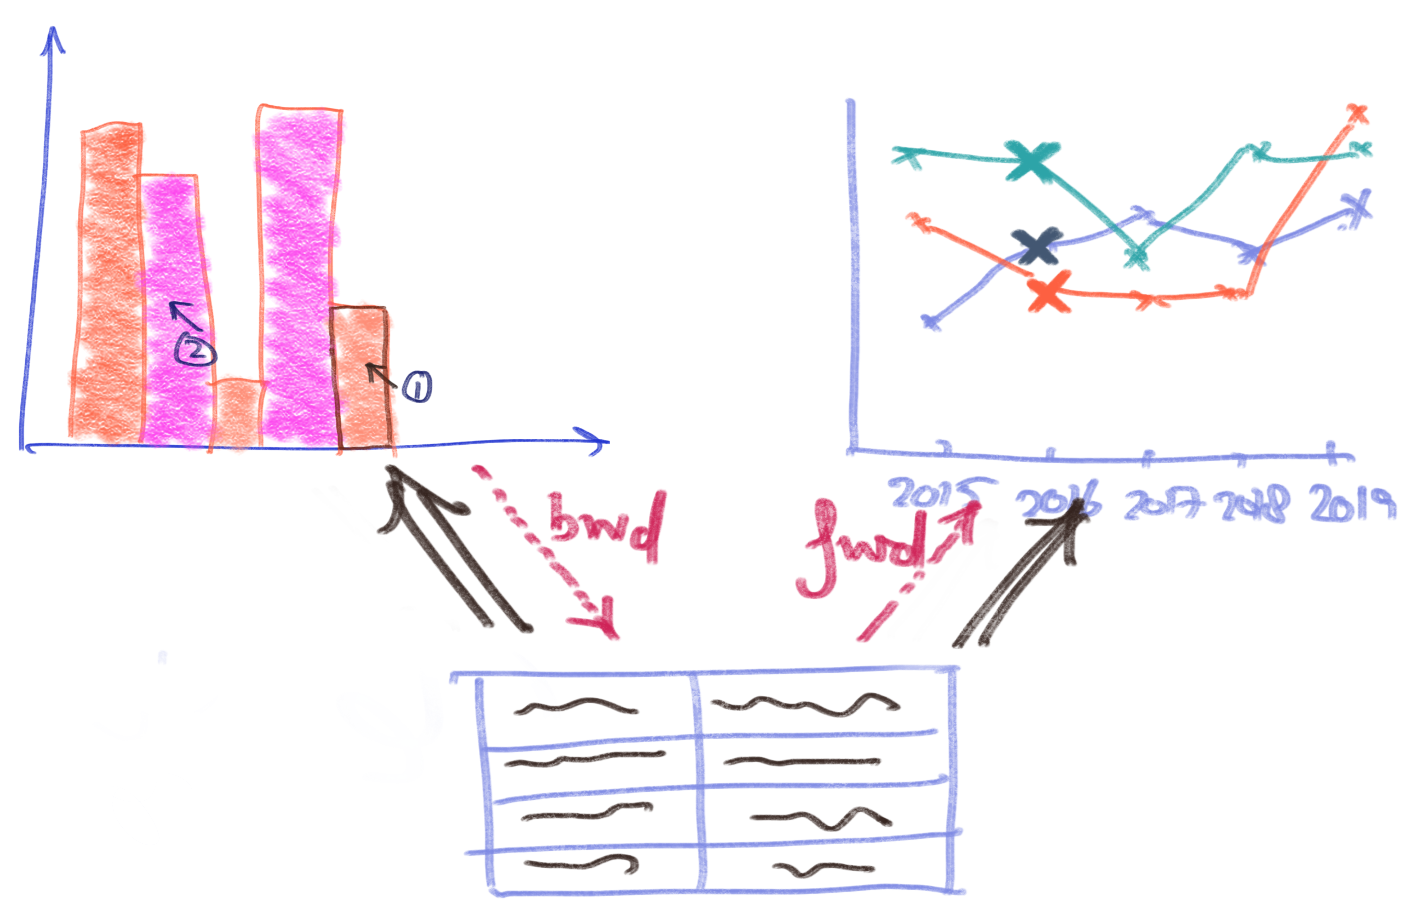
\includegraphics[scale=0.14]{fig/example/vis-linking.png}}
   \small
   \begin{lstlisting}
     let input = [ ... ]
     let b1 = input |> filter (fun c -> c.country = "AB")
     let b2 = input |> filter (fun c -> c.country = "CD")
     let bc = barchart [b1; b2]
     let lc = input |> some filter |> linechart
   \end{lstlisting}
   \todo{TP: Tweaked code to look a bit more like what I think we'd need.}
   \caption{Linking visualisations via common data dependencies}
   \label{fig:introduction:vis-linking}
\end{figure}

We can again frame this as a program analysis problem. It is a matter of selecting a part of the structured output and performing a backwards analysis to identify the required inputs, as before, but then performing a further forwards analysis to identify dependent parts of the other output. This is also shown in \figref{introduction:vis-linking} above. This would provide a language-based foundation for brushing and linking, allowing it to be automatic and pervasive, but also ``data-transparent'', able to provide a concise view of the data that underpin a given relationship.

\subsection{Contributions}

To solve these problems, we need a dependency analysis which supports focusing on substructures of rich outputs, and moreover one which can be used bidirectionally, with appropriate round-tripping properties. Recent program slicing techniques \cite{perera12a,perera13a,ricciotti17} allow the user to focus on the output by ``erasing'' parts deemed to be irrelevant; the erased parts, called \emph{holes}, are propagated backwards by a backwards analysis which identifies parts of the program and input which are no longer needed. Although these approaches enjoy useful round-tripping properties characterised by Galois connections, they only allow focusing on \emph{prefixes} of a structured output, rather than arbitrary substructures.

In this paper, we present new language-based data provenance techniques for linking structured outputs, such as visualisations, to structured inputs, and to each other, in a fine-grained way. Our specific contributions are as follows:

\begin{itemize}[leftmargin=*]
   \item[--] a review of \emph{Galois slicing}, a program slicing framework with round-tripping properties appropriate to our problem, and an analysis of its shortcomings (\secref{background});
   \item[--] a new bidirectional dependency analysis inspired by Galois slicing, addressing these shortcomings, for a core calculus with lists and arrays, and a discussion of how the analysis can be used in various ways to link inputs to outputs and outputs to other outputs (\secref{core-language});
   \item[--] a richer surface language called \OurLanguage with familiar functional programming features, including piecewise definitions, pattern matching, list notation and list comprehensions, and an extension of our analysis to the desugaring (\secref{surface-language});
   \item[--] an implementation of Fluid in PureScript, and a discussion and evaluation of the strengths and weaknesses of our approach (\secref{implementation}).
\end{itemize}
